\documentclass[10pt,a4paper]{article}
\usepackage[latin1]{inputenc}
\usepackage{amsmath}
\usepackage{amsfonts}
\usepackage{amssymb}
\usepackage{graphicx}

\author{Group 16}
\title{Titan Expedition\\ Project 1.2 - Report}
\usepackage{titlesec}

%No idea about how this works, it is used to have numbered paragraphs
\setcounter{secnumdepth}{4}
\setcounter{tocdepth}{4}
\titleformat{\paragraph}
{\normalfont\normalsize\bfseries}{\theparagraph}{1em}{}
\titlespacing*{\paragraph}
{0pt}{3.25ex plus 1ex minus .2ex}{1.5ex plus .2ex}


\begin{document}
	\begin{titlepage}	
		\begin{center}	
		{\LARGE Maastricht University}\\
		\vspace{15pt}
		{\large Department of Data Science and Knowledge Engineering}
		\vspace{30pt}
		
		\hrule
		\vspace{15pt}
		{\Large Titan Expedition}\\
		\vspace{15pt}
		{\large Project 1-2 - Report}
		\vspace{15pt}
		\hrule
		
		\vspace{30pt}
		Group 16\\
		\vspace{15pt}
		
		\textit{Authors:}\\
		Jan-Felix De Man (i6201411)\\
		Selim Gilon (i6192074)\\
		Gyumin Oh ()\\
		Pietro Piccini (i6188338)\\
		Gianluca Vico (i6183186\\			
		\vspace{15pt}
		
		\textit{Supervisors:}
		...\\
		\vspace{15pt}
		
		\textit{Examiners:}
		...\\
		\vspace{15pt}
		
		\vspace*{\fill}
		Block 1.6\\
		Bouillonstraat 8-10, 6211 LH Maastricht, Netherlands\\
		27 July 2019
		\end{center}
	\end{titlepage}

	\newpage
	\section*{Preface}
	
	\begin{abstract}
	Bla bla bla with footnote \footnote{Bla bla bla footnote}	
	\end{abstract}

	\newpage
	
	\tableofcontents
	\newpage
	
%%%%%%%%%%%%%%%%%%%%%%%%%
	\section{List}
	\subsection{Abbreviations}
	Bla bla bla
	\subsection{Tables}
	Bla bla bla
	\subsection{Figures}
	Bla bla bla
	
%%%%%%%%%%%%%%%%%%%%%%%%%%
	\section{Introduction}

	\subsection{Problem description}

	\subsection{Research questions}

	\subsection{Report structure}

%%%%%%%%%%%%%%%%%%%%%%%%%	
	\section{Models}

	\subsection{Solar System}
	\subsubsection{Physical approach and alternatives}
	To digitally simulate our solar systems we used Newton's gravitational theorem. The model is based on equation $\vec{F} = \frac{\vec{r}}{|\vec{r}|} G \dfrac{m_1 m_2}{|\vec{r}|^2} $ \footnote{(2019). Retrieved from https://www3.nd.edu/~zxu2/acms40390F15/Lec-5.6.pd}, this means that the gravitational force F is equal to the product of the masses of both objects, divided by the distance squared, multiplied by the gravitational constant G. Or in other words: the bigger the mass and the closer the distance, the bigger the force.\\
	To implement this model, it is necessary to pick a certain point in time and  to know where the planets were located at that time. Once all the celestial bodies are loaded in their original place, the gravity will do its work, which results in the planets orbiting around the Sun and the moons around their respective planets.\\ \\
	
	Another possibility was to simulate our solar system using an orbital model. This approach is simpler: draw the sun and surround it with ellipses that represent the size of the orbits of the planets. \\
	Newton's model has been chosen instead of the orbital model, because more physically accurate and it can show the evolution of the Solar System. Moreover it only needs the initial conditions of each body and the gravitational formula. On the other hand calculating the position of a body at a given time could be tricky and the complexity of the algorithm increases exponentially if the number of bodies in the simulation increases. 
	
	\subsubsection{Equation solvers}
	The whole simulated solar system works on just equation: Newton's gravitational theorem. In order to implement this and actually make the celestial bodies orbit, you have to solve this equation. There are multiple ways to do it, represented are the ones used in the making of this report.
	
	\paragraph{Euler}
	Euler's method is a numerical method that solves first order first degree differential equations. It is one of the most simple ODE-solvers, yet still relatively accurate. 
	\begin{flalign}
	&\dot{y}(t) = f(t, y)\\
	&y_i \approx w_i = w_{i - 1} + hf(t_{i -1}, w_{i-1}),\ \text{with}\ i > 0
	\end{flalign}
	This methods as a global error $O(h)$, require only one function evaluation at each iteration and it is easy to implements.
	
	\paragraph{Adams-Bashforth}
	We decided to use Adams-Bashforth explicit 4 steps method to solve the different equations. 
	This method has been implemented and replaced the Euler's method to have a higher accuracy in the calculus of the simulation. As mentioned earlier, Euler's method is first order while Adams-Bashforth is a 4rth order equation solver. Adams-Bashforth's method is more accurate than Euler's, that is why it is recommended to work with the Adams-Bashforth method. 
	This method is defined as
	\begin{flalign}
	&\dot{y}(t) = f(t, y)\\
	&y_{i + 1} \approx w_{i + i} = w_i + \frac{h}{24} [55f(t_{i}, w_{i}) - 59 f(t_{i -1}, w_{i-1}) + 37 f(t_{i -2}, w_{i-2}) - 9 f(t_{i -3}, w_{i-3})],\ \text{with}\ i > 3
	\end{flalign}
	To initialize this method, data from Nasa are used if available. The acceleration is calculated by using 3 points difference formula and data for the spaceship are assumed to be linear.\\
	The main advantage of the approach is that it reduces the error (from O(h) for Euler's to O(h4) for Adams-Bashforth's) without increasing the computational cost, because both of the require only a function evaluation at each iteration.	
	
	\paragraph{3 point difference}
	It was not possible to obtain information about the acceleration of the celestial bodies from Nasa, so it is necessary to calculate it. The acceleration is defined as $\vec{a} = \frac{d\vec{v}}{dt} $. So the values of the acceleration can be calculated as following:
	
	\begin{flalign}
		\text{Forward difference: } &\vec{a}_i = \dfrac{-3\vec{v}_i + 4\vec{v}_{i + 1} - \vec{v}_{i + 2}}{2h}\\
		\text{Centered difference: } &\vec{a}_i = \dfrac{\vec{v}_{i + 1} - \vec{v}_{i - 1	}}{2h} \\
		\text{Backward difference: } &\vec{a}_i = \dfrac{3\vec{v}_i - 4\vec{v}_{i - 1} + \vec{v}_{i - 2}}{2h}
	\end{flalign}
	
	\paragraph{Error analysis}	

	\subsection{Spaceship}
	\subsubsection{Shape}
	Our rocket is designed to be a spherical shell that is hollow inside. This makes it easier to calculate forces caused by external factors, such as wind and pressure, that affect the rocket. The effects of the wind is determined by the surface area: that more area that can be blown by the wind, the bigger the force. The choice of this shape, although not the most aerodynamic, which leads to increased costs, does help to control the rotation, increases the shuttle's stability and efficiency.
	
	\subsubsection{Engines and uses}
	Our rocket is uses 7 engines which control velocity and rotation. The engines are divided into 2 categories: 1 main engine and 6 sub engines. Main engine allows us to control the rocket's velocity and acceleration. The sub engines change the rotation of our vehicle for the different axis x, y, z. For every axis, or dimension, we have 2 sub engines or thrusters. This helps us establish better control over our rocket. This is very important in the case of heavy winds.
	Main engine acceleration / deceleration; thrusters to balance out wind.
	
	\subsubsection{Rotation}
	Spaceship's rotations are calculated from torque momentum formula = r F, where r is the distance between the application point of the force and the center of the spaceship, and the angular momentum formula $ \vec{L} = I \vec{\omega}$. Because of the particular shape of the spaceship inertia momentum is $I = \frac{2}{5}m \dfrac{r^5_2 - r^5_1}{r^3_2 - r^3_1}$. Then the angular velocity could be approximated as $\vec{\omega} = \dfrac{\sum_{i = 0}^{n}(\vec{r}_i \times \vec{F}_i)\Delta t}{I} $ and the rotation is $\vec{\theta} = \frac{d\vec{\omega}}{dt} $, which is calculated with Adams-Bashforth's method.\\
	To calculate the orientation of the spaceship three perpendicular axis are used: $x$ and $y$ are horizontal and $z$ is the vertical one. Orientation is computed by using axis-angle rotations: given the unit axis of rotation $\vec{e}$ and the angle $\theta$, the axis of the spaceship are updated to 
	\begin{equation}
		\vec{v}^* = (\cos\theta)\vec{v} + (\sin\theta)(\vec{e} \times \vec{v}) + (1 - \cos\theta)(\vec{e} \cdot \vec{v}) \vec{e}
	\end{equation}
	
	
%%%%%%%%%%%%%%%%%%%%%%%%%%%%
	\section{Travel}
	\subsection{Launch}
	\subsubsection{From Earth}
	For the launch on Earth we use the same point in time as we initialize our digital Solar System, which is the 22nd of March 2019 at midnight. We launch from really close to the equator (latitude -0.0016�) facing Titan
	\subsubsection{From Titan}
	
	\subsection{Trajectory}
	The trajectory is determined by the starting velocity of the rocket and the gravity influenced on the rocket by the celestial bodies in the solar system, according to Newton's gravitational theorem (see 3.1.1.).
	
	\subsubsection{Algorithm}
	To find a trajectory we developed an algorithm that finds the initial vector velocity of the rocket such that the rocket reaches Titan's atmosphere. The algorithm works by launching the rocket towards Titan with a generic initial velocity. After a determined amount of time the rocket stops and the vector distance between the rocket and Titan is stored and used to correct the rocket's initial velocity, then it is launched again with the improved initial velocity. This process is repeated and the correction made to the initial velocity is proportional to the distance between the rocket and Titan at the end of the launch. This is useful to avoid over-correcting and guarantees that the rocket will find a trajectory after a finite number of iterations. Moreover the correction factor is changed when the rocket can go close to Titan, in this way it oscillates less around the optimal solution and converges faster.
		
	\subsubsection{To Titan}
	\subsubsection{To Earth}

%%%%%%%%%%%%%%%%%%%%%%%%%%%%%
	\section{Landing}
	When the shuttle managed to orbit around the target planet, it will start an automated landing. The landing is coordinated by two built-in controllers. These algorithms help to land our shuttle safely on the surface of the planet.
	\subsection{On Titan}
	\subsubsection{Given tolerances}
	In order to assure a safe landing, it is required to respect multiple parameters. A landing is considered safe when the velocity is less than 0.1, the angular velocity less than 0.01, the angle between the vertical axis of the spaceship and the ground is less than 0.02 and the distance to the ground less than 0.1.
	
	\subsubsection{Stochastic wind model}
	\subsubsection{Feedback controller}
	\subsubsection{Open loop controller}
	The computation for the velocity during the landing is done by using an open loop controller: at 50'000 km the velocity is reduced to 500 km/h (with respect to Titan) with the main engine and with the same direction of the velocity of Titan. Then at 600km, when the spaceship enters the atmosphere, it starts braking to have the same velocity of the planet. During this phase the feedback controller for the rotation is still working and a three dimensional space is used.
	
	\subsection{On Earth}

%%%%%%%%%%%%%%%%%%%%%%%%%%%		
	\section{Optimizations}
	\subsection{Fuel efficiency}
	Every time that the spaceship uses its engines it consume fuel, so it reduces its mass. The total mass at the launch is 20'000 kg, 15'000 kg are fuel. When it lands on Titan it has consumed 5529.55 kg of fuel. The cost of the fuel is assumed to be the same of kerosene (1.68 ? / gallon \footnote{Jet Fuel - Monthly Price (Euro per Gallon) - Commodity Prices - Price Charts, Data, and News - IndexMundi. Retrieved from https://www.indexmundi.com/commodities/?commodity=jet-fuel\&months=12\&currency=eur}, about 0.55 ? / kg), then the cost is about ? 3067.58. The estimate of the cost when the rocket start the landing at 50'000 km from Titan is ? 1181.00. The estimation assumes that there are no rotation nor atmosphere and it calculates the constant acceleration needed to land with a null  velocity and a distance of zero meters from the ground. 
	From constant acceleration motion formula it is possible to derive that $\vec{a} = \frac{|\vec{v}|^2}{2h}$, where $h$ is the distance from the ground. Then the mass $M$ of fuel need is $M = \dfrac{m a}{F_{engine}}m_{engine} $ and the cost is calculated by using the mass M.
	
	
	\subsection{Quickest route to Titan}
	\subsection{Math optimizations}

%%%%%%%%%%%%%%%%%%%%%%%%%%
	\section{GUI}
	The program described in this report calculates everything in the three dimensions. The solar system it simulates is visualized in 3D. There are added functionalities to make this program more user-friendly: use the buttons A and D to rotate the camera view, press 0 to reset it to the standard rotation. The buttons W and S can be used respectively to zoom in and out. If you press E, the camera will be focused on Earth, T will focus on Titan, U will set the view to Saturn. Furthermore you can use the arrow keys to roam around freely in space.\\ \\
	
	As soon as we initialize our landing, the GUI switches to a 2D visualization of our rocket landing on the celestial body. All the calculations it uses are still made in three dimensions. You can see the spherical-shaped rocket getting closer to the planet's surface, while it gets affected by the wind. You see the rocket correcting its rotation and speed before it hits the surface.
	
%%%%%%%%%%%%%%%%%%%%%%%%%%	
	\section{Experiments}
	Since our rocket travels with a speed of approximately 56'118 km/h, we experimented with lower speeds to make it more realistic. To do so, the initial velocity with which the rocket is launched has been reduced. When changing the velocity to realistic speeds, the shuttle ended up orbiting around the Sun, or sometimes even worse, Earth itself. But if the speed is realistic, then why does not it work in this simulation? In this case, the rocket is shot into space from our launching station, and does not use its engines until it reaches the orbit of the desired celestial body. Therefore it will get stuck in the orbit of either the Sun or Earth. In real life, a rocket uses its own engine to leave Earth orbit and to steer itself to its desired location. Simulating this process would mean that you would need to rethink your whole launching and trajectory approaches, thus would be very time consuming. We see this as a challenge we would like to work on later. 
	
	Since our wind model rightfully predicts a low wind on the surface, we wanted to test the controller for stormier weather as well. We did find data about the wind on Titan and Earth, but we do not want to be surprised by having our rocket crash after all the effort we put into getting it to the planet. 
	
%%%%%%%%%%%%%%%%%%%%%%%%%%
	\section{Results and discussion}
	It is possible to test how robust is the feedback controller by increasing the effect of the rotations generated by the wind.
	\\
	\vspace{10pt}
		
	\begin{tabular}{|c||c|c|c|c|}
		\hline
		Rotation influence & x1 & x10 & x100 & x1000 \\
		\hline \hline
		Angular velocity (rad/s) & 0.0012 & 0.0099 & 0.0755 & 0.8471 \\ 
		\hline 
		Angle (rad) & 0.0093 & 0.0093 & 0.0093 & 0.0092 \\ 
		\hline 
	\end{tabular} 
	\\
	\vspace{10pt}
	\\
	Then the values of the angular velocity and the angle of the spaceship are within the tolerance range, even with rotations 1000 times stronger.\\
	It is possible to reduce the initial velocity of the spaceship from Earth to test if it can land.
	\\
	\vspace{10pt}
	
	\begin{tabular}{|c||c|}
		\hline 
		Velocity compared  to optimal & Result - cost (?) \\ 
		\hline \hline
		99\% & Fail \\ 
		\hline 
		99.9\% & Fail (in Titan gravitational field) \\ 
		\hline 
		100\% & 3067.58 \\ 
		\hline 
		100.1\% & Fail (in Titan gravitational field) \\ 
		\hline 
		101\% & Fail \\ 
		\hline 
	\end{tabular} 
	\\
	\vspace{10pt}\\
	Then trajectory is really sensitive to the initial conditions and the spaceship completely miss Titan if there are small changes at the beginning. The velocities used have the same direction of the optimal one.
	
%%%%%%%%%%%%%%%%%%%%%%%%%%	
	\section{Conclusion}
	
	%Future improvements
	We are planning to search for a more realistic launching velocity by using other celestial bodies to improve the trajectory (in particular Jupiter seems promising) and by organizing a longer travel, for example a 8-year-long travel similar to Cassini mission. 
	Then it is possible to improve the orbit around Titan: at the moment the spaceship can complete a few orbits around the satellite, but because of the speed and the Saturn gravitational force it cannot stay longer. By reducing the velocity it will be possible to orbit longer.
	A feedback controller that tries to reduce the distance between Titan and the spaceship can used, this way it is possible to reduce the landing velocity more and to have a more realistic landing.
	Finally it is possible to explore other numerical methods to improve the accuracy of the whole simulation.
	
	\section*{Bibliography}
	\begin{enumerate}		
		\item Rincon, P. (2005). BBC NEWS | Science/Nature | Huygens sends first Titan images. Retrieved from http://news.bbc.co.uk/2/hi/science/nature/4175099.stm\ [Accessed 6 May 2019].
		
		\item Bortman, H. (2010). Life Without Water And The Habitable Zone. \\Retrieved from\\ http://www.spacedaily.com/reports/Life\_Without\_Water\_And\_The\_Habitable\_Zone\_999.html [Accessed 4 May 2019].
		
		\item Bartels, M. (2019). NASA May Decide This Year to Land a Drone on Saturn's Moon Titan. Retrieved from https://www.space.com/43010-dragonfly-mission-would-put-a-drone-on-titan.html [Accessed 17 June 2019].

		\item Retrieved from https://www3.nd.edu/~zxu2/acms40390F15/Lec-5.6.pdf [Accessed 1 May 2019].

		\item Hendrix, A. and Yung, Y. (2017). Energy Options for Future Humans on Titan. [online] Available at: https://arxiv.org/ftp/arxiv/papers/1707/1707.00365.pdf [Accessed 2 May 2019].
		
		\item Carey, B. (2005). New View of Titan: Strong Winds, Soft Ground and Lightning. Retrieved from https://www.space.com/1825-view-titan-strong-winds-soft-ground-lightning.html [Accessed 3 May 2019]
		
		\item Jet Fuel - Monthly Price (Euro per Gallon) - Commodity Prices - Price Charts, Data, and News - IndexMundi. Retrieved from \\https://www.indexmundi.com/commodities/?commodity=jet-fuel [Accessed 18 June 2019].		
	\end{enumerate}

	\newpage
	\section*{Appendix}
	\begin{figure}[h]
		\centering
		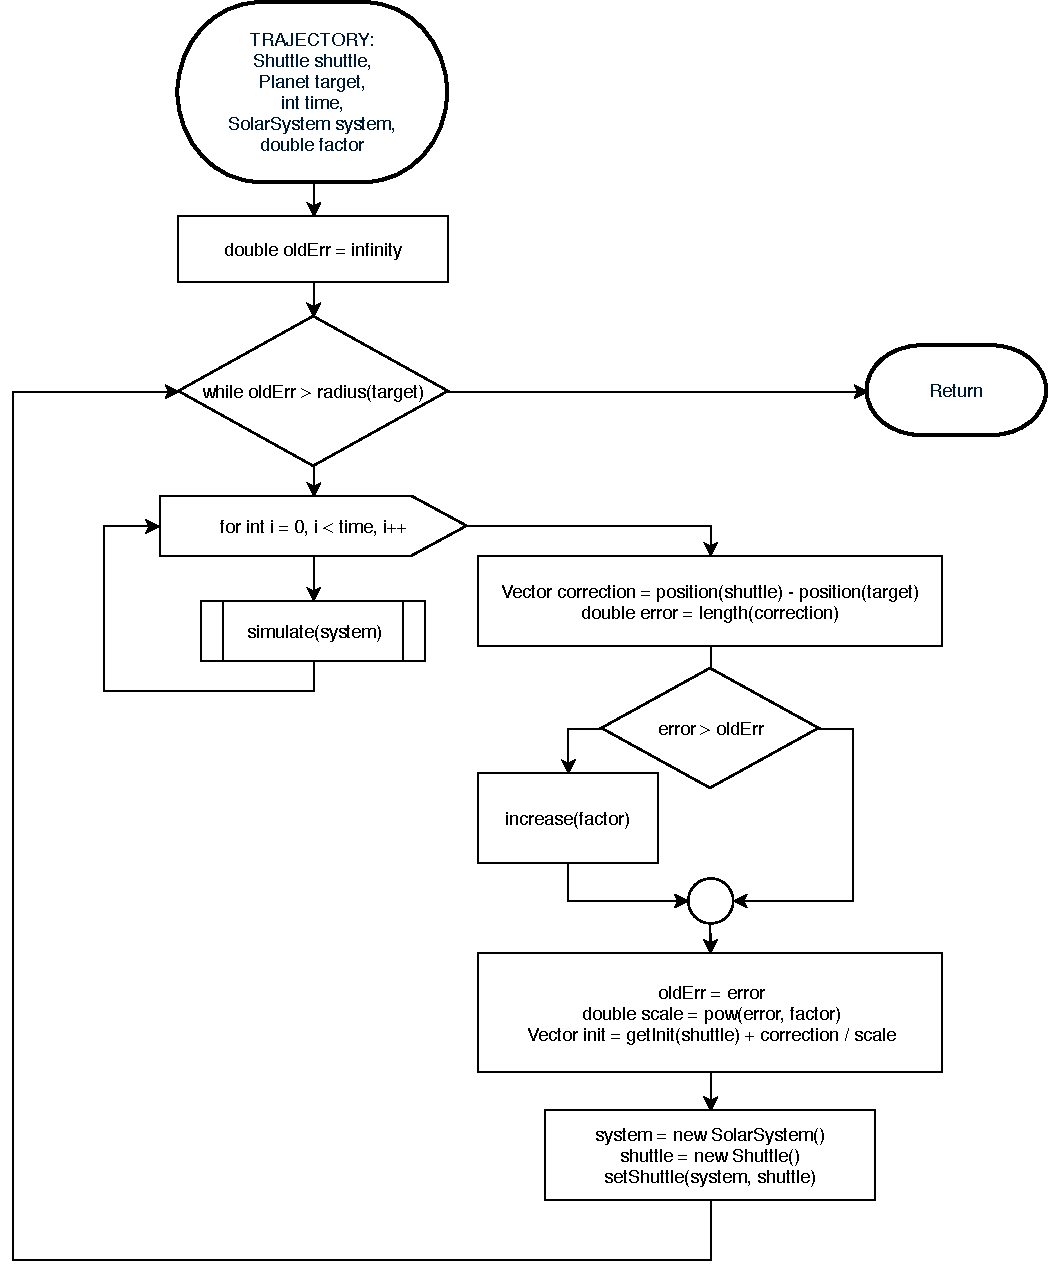
\includegraphics[width=1\linewidth]{trajectory}
		\caption[Short]{Algorithm to calculate the trajectory to reach a planet.}
		\label{fig:trajectory}
	\end{figure}
	
\end{document}